\documentclass[12pt,a4paper]{article}
\usepackage[a4paper,top=1.5cm, bottom=1.5cm, left=1.5cm, right=1.5cm]{geometry}
\usepackage[T2A]{fontenc}
\usepackage[utf8]{inputenc}
\usepackage[russian]{babel}
\usepackage{amsmath}
\usepackage{amssymb}
\usepackage{graphicx}
\usepackage{floatrow}
\usepackage{booktabs}
\usepackage{wrapfig}
\usepackage{indentfirst}
\usepackage{lipsum}
\usepackage{subcaption}
\usepackage{float}
\usepackage{enumitem}
\restylefloat{table}

\newcommand{\figref}[1]{(см. рис. \ref{#1})}
\newcommand{\e}[1]{\text{$\cdot10^{#1}$}}

\title{Лабораторная работа 5.10.1 \\ Электронный парамагнитный резонанс}
\author{Симанкович Александр\\ Б01-108}
\date{15.10.2023}

\begin{document}
	\maketitle
	
	\section*{Аннотация}
	
	В работе экспериментально подтвержден эффект электронного парамагнитного резонанса в молекуле дифенилпикрилгидразила (ДФПГ). Подтверждена теоретическая зависимость резонансной частоты от значения магнитного поля. Получен $g$-фактор несвязанного электрона в молекуле ДФПГ $g = (1.94 \pm 0.04)$ . Оценено время релаксации электрона в молекуле ДФПГ $\tau = (15.0 \pm 1.0)$ нс.
	
	\section*{Теоретическое введение}
	
	\subsection*{Основы ЭПР}
	
	\begin{wrapfigure}[15]{r}{7.0cm}
		%              ^^ number of occupied rows
		\includegraphics[scale=0.6]{res/epr.png}
		\caption{Конфигурация полей и магнитного диполя.}
		\label{fig:epr_theory}
		\vspace{0pt}
	\end{wrapfigure}

	В присутствии внешнего магнитного поля энергетический уровень электрона расщепляется на два подуровня, разность энергий между которыми
	$$ \Delta E = 2 \mu B, $$
	где $\mu$ -- проекция магнитного момента на направление поля.

	Переходы между этими двумя уровнями могут возбуждаться внешним электромагнитным полем, если его вектор магнитной индукции перпендикулярен расщепляющему полю, а энергия его квантов равна разности $\Delta E$:
	\begin{equation}
		\hbar \omega_0 = 2 \mu B,
		\label{eq:frequency}
	\end{equation}
	где $\omega_0$ -- резонансная частота. Это являение называется \textit{электронным парамагнитным резонансом} (ЭПР).
	
	В большинстве веществ электроны находятся в спаренном состоянии и "переворот" спина невозможен. ЭПР наблюдается только на неспаренных электронах, которые, как известно, определяют свойство парамагнетизма вещества.
	
	Для электрона выполняется гиромагнитное соотношение:
	\begin{equation}
		\frac{\vec{\mu}}{\mu_{\text{Б}}} = \frac{g \vec{M}}{\hbar} \quad \Rightarrow \frac{\mu}{\mu_{\text{Б}}} = \frac{g s \hbar}{\hbar},
	\end{equation}
	где $\vec{M}$ -- момент импульса, $s = 1/2$ -- спин электрона, $\mu_{\text{Б}} = \frac{e \hbar}{2 c m_e}$ -- магнетон Бора, $g$ -- $g$-фактор.
	
	Тогда $g$-фактор выражается как:
	\begin{equation}
		g = \frac{\hbar \omega_0}{\mu_{\text{Б}} B}.
		\label{eq:g_factor}
	\end{equation}
	
	\subsection*{Релаксация}
	При перевороте всех спинов энергия должна прекратить поглощаться. Но этого не происходит, поскольку есть процессы безызлучательного рассеяния энергии: спин-решеточная и спин-спиновая релаксации.
	
	В равновесном состоянии распределение электронов по уровням подчиняется распределению Больцмана:
	$$ \frac{N_{\text{в}}}{N_{\text{н}}} = e^{- \Delta E / k_{\text{Б}} T}. $$
	
	Под действием внешнего электромагнитного излучения это равновесие нарушается. За счет взаимодействия электронов с другими электронами (спин-спиновое) и решеткой вещества (спин-решеточное) они передают поглощенную энергию в кинематические степени свободы.
	Отметим, что термин "решетка" не ограничивает нас лишь твердым агрегатным состоянием. Любое взаимодействие спинов с термодинамически равновесной системой является спин-решеточным взаимодействием. Поэтому термин применим и для жидкостей, газов.
	
	Оценим время релаксации через соотношение неопределенностей:
	\begin{equation}
		\Delta E \approx \frac{\hbar}{\tau}.
		\label{eq:relaxation}
	\end{equation}
	
	\subsection*{ДФПГ}
	
	\begin{figure}[H]
		\centering
		\begin{minipage}{0.6\textwidth}
			\centering
			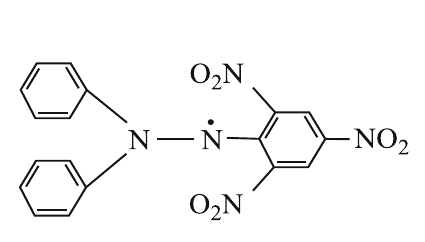
\includegraphics[width=0.7\linewidth]{res/dfpg_struct.png}
		\end{minipage}%
		\begin{minipage}{0.4\textwidth}
			\centering
			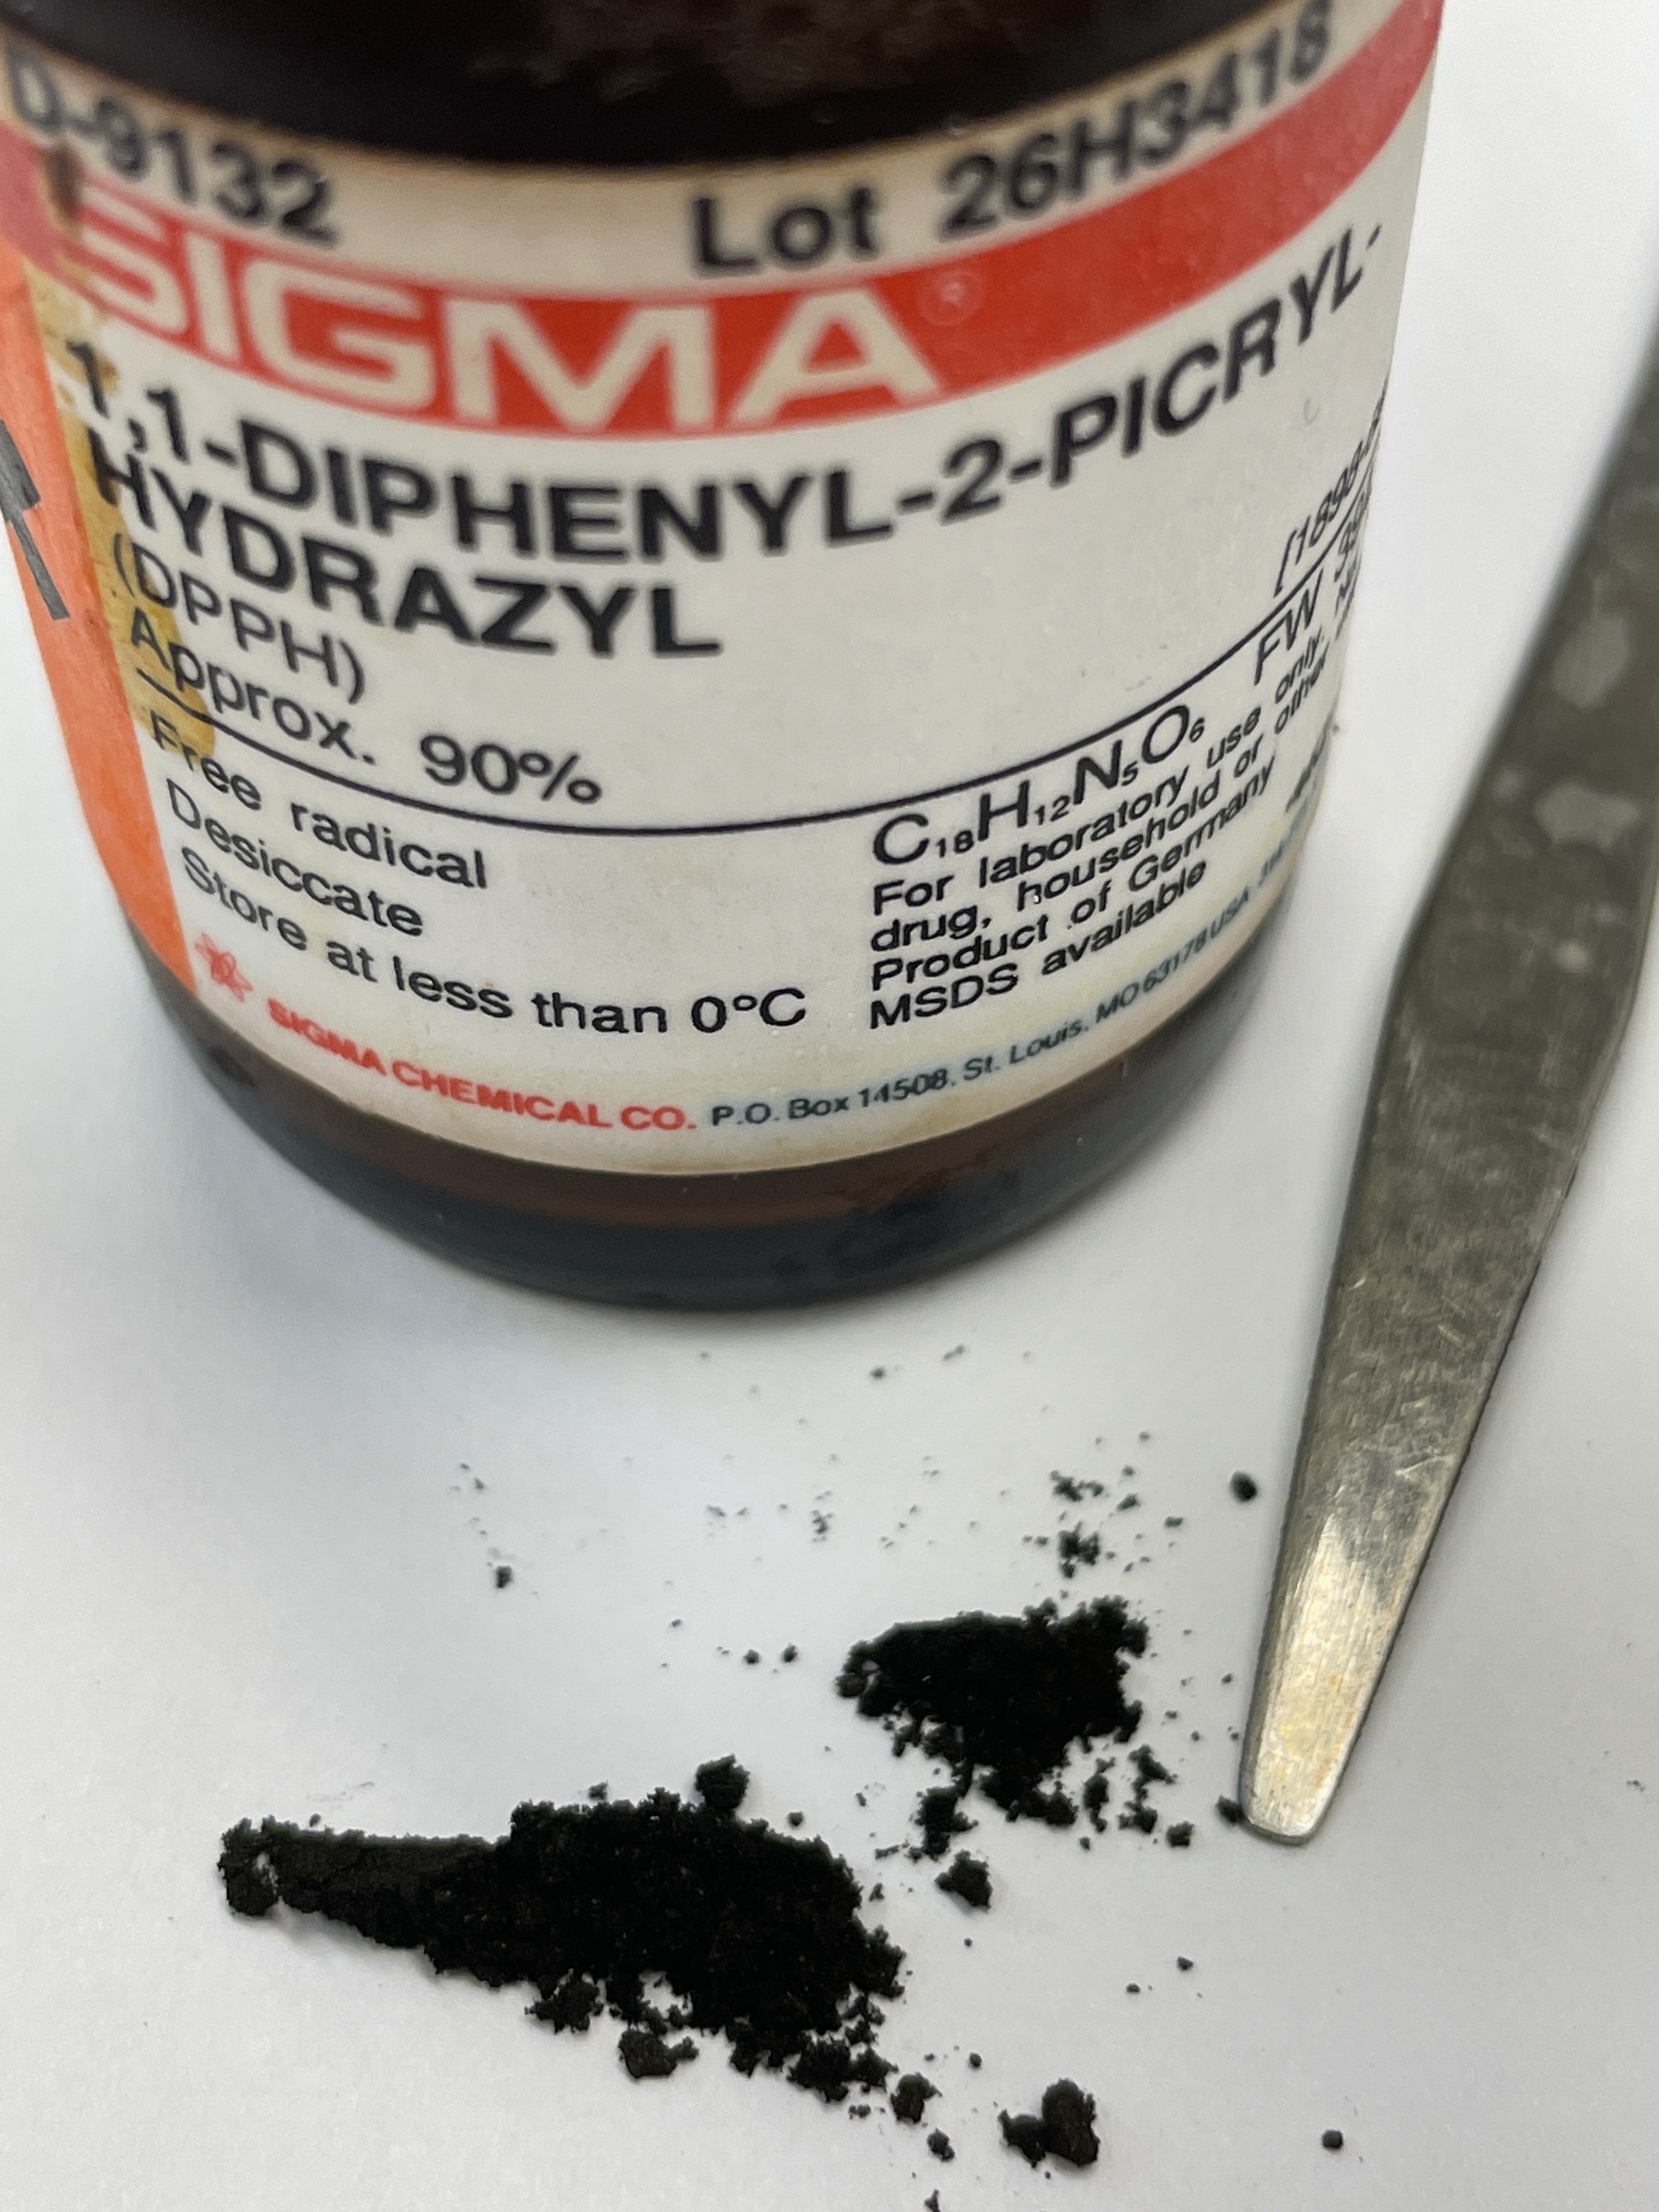
\includegraphics[width=0.7\linewidth]{res/dfpg.jpg}
		\end{minipage}
		\caption{Дифенилпикрилгидразил. Слева: структурная формула. Справа: образец ДФПГ.}
		\label{fig:dfpg}
	\end{figure}
	
	ДФПГ представляет собой органическую молекулу с одним неспаренным электроном атома азота $N$. Чисто спиновый магнетизм ДФПГ (почти отсутствует орбитальный магнетизм) приводит к тому, что парамагнитный резонанс происходит почти как на свободных электронах, что дает оценку $g = 2.00$.
	
	\section*{Методика эксперимента}
	
	\begin{figure}[H]
		\centering
		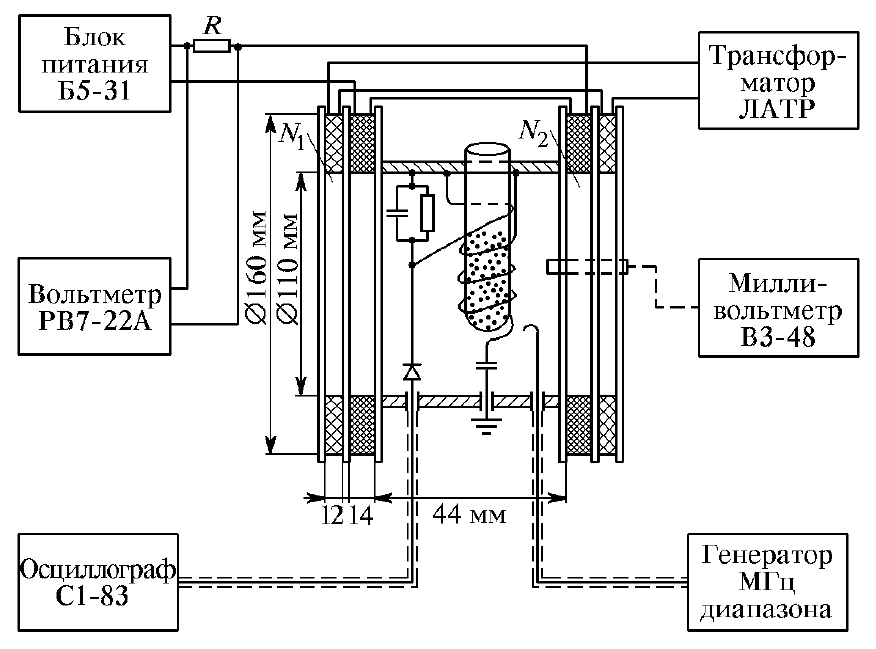
\includegraphics[width=0.6\linewidth]{res/scheme.png}
		\caption{Схема установки для изучения ЭПР.}
		\label{fig:setup}
	\end{figure}
	
	\begin{figure}[H]
		\centering
		\begin{minipage}{0.5\textwidth}
			\centering
			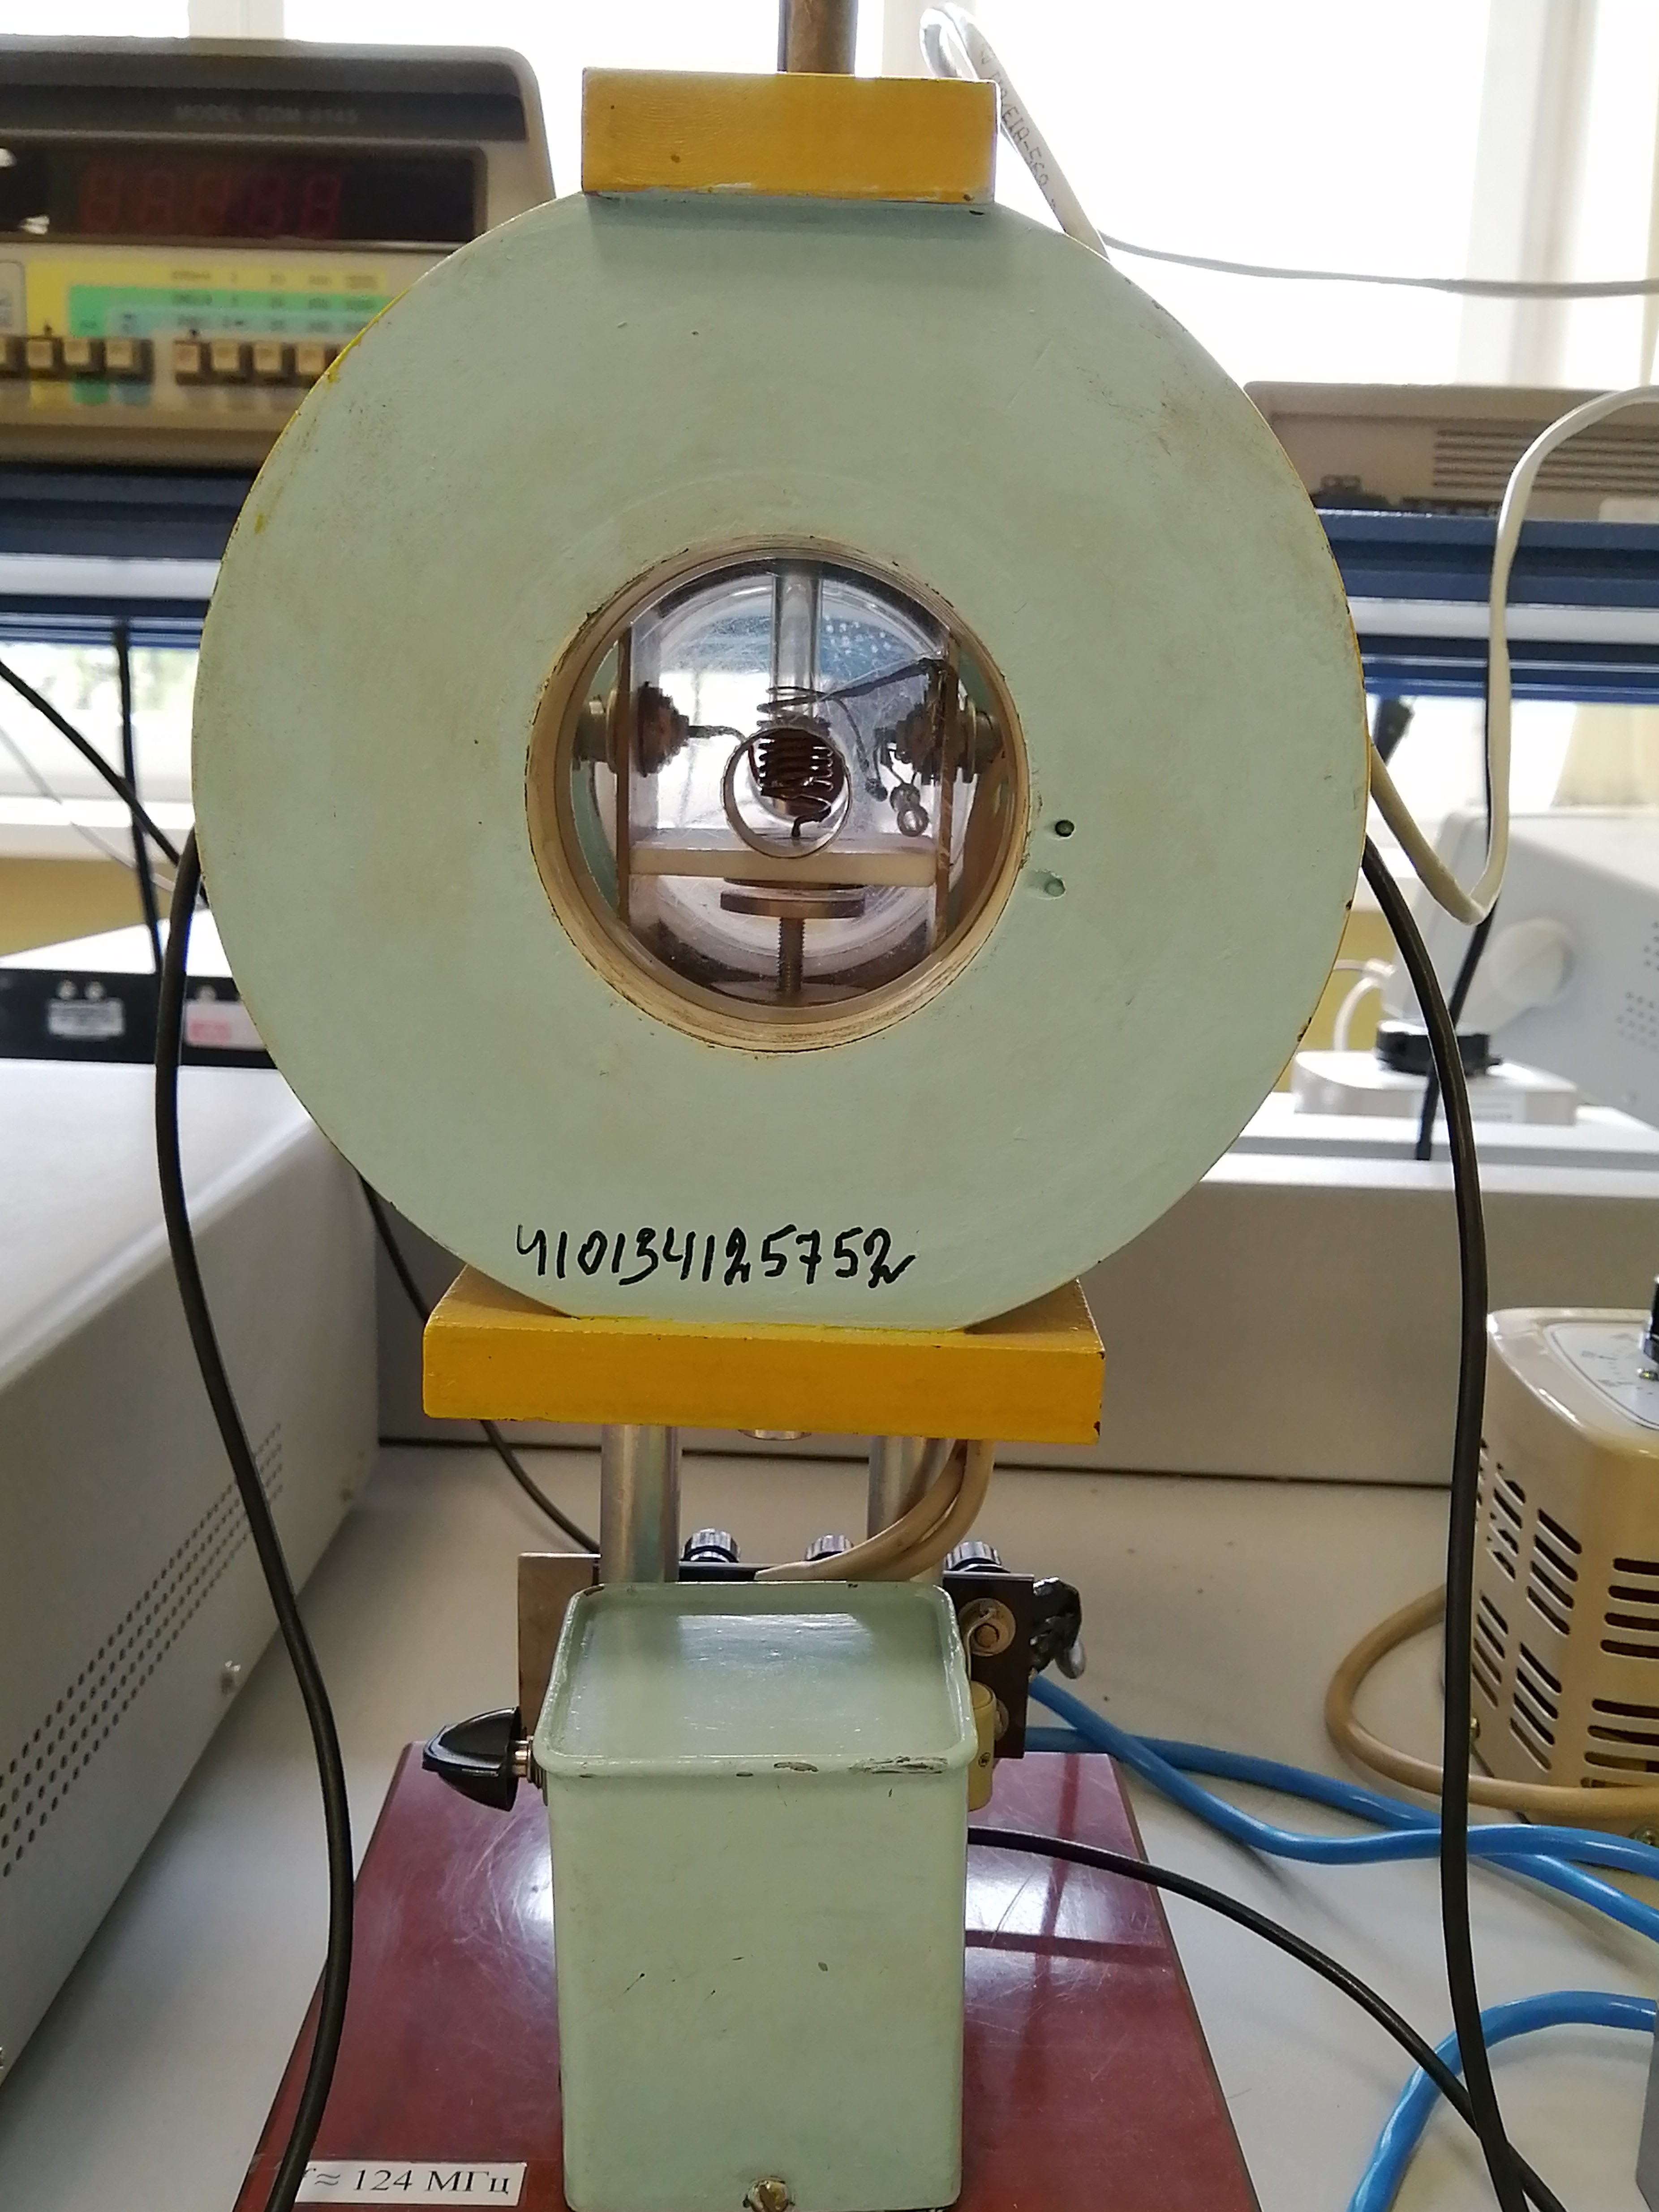
\includegraphics[width=0.7\linewidth]{photos/coil_front.jpg}
		\end{minipage}%
		\begin{minipage}{0.5\textwidth}
			\centering
			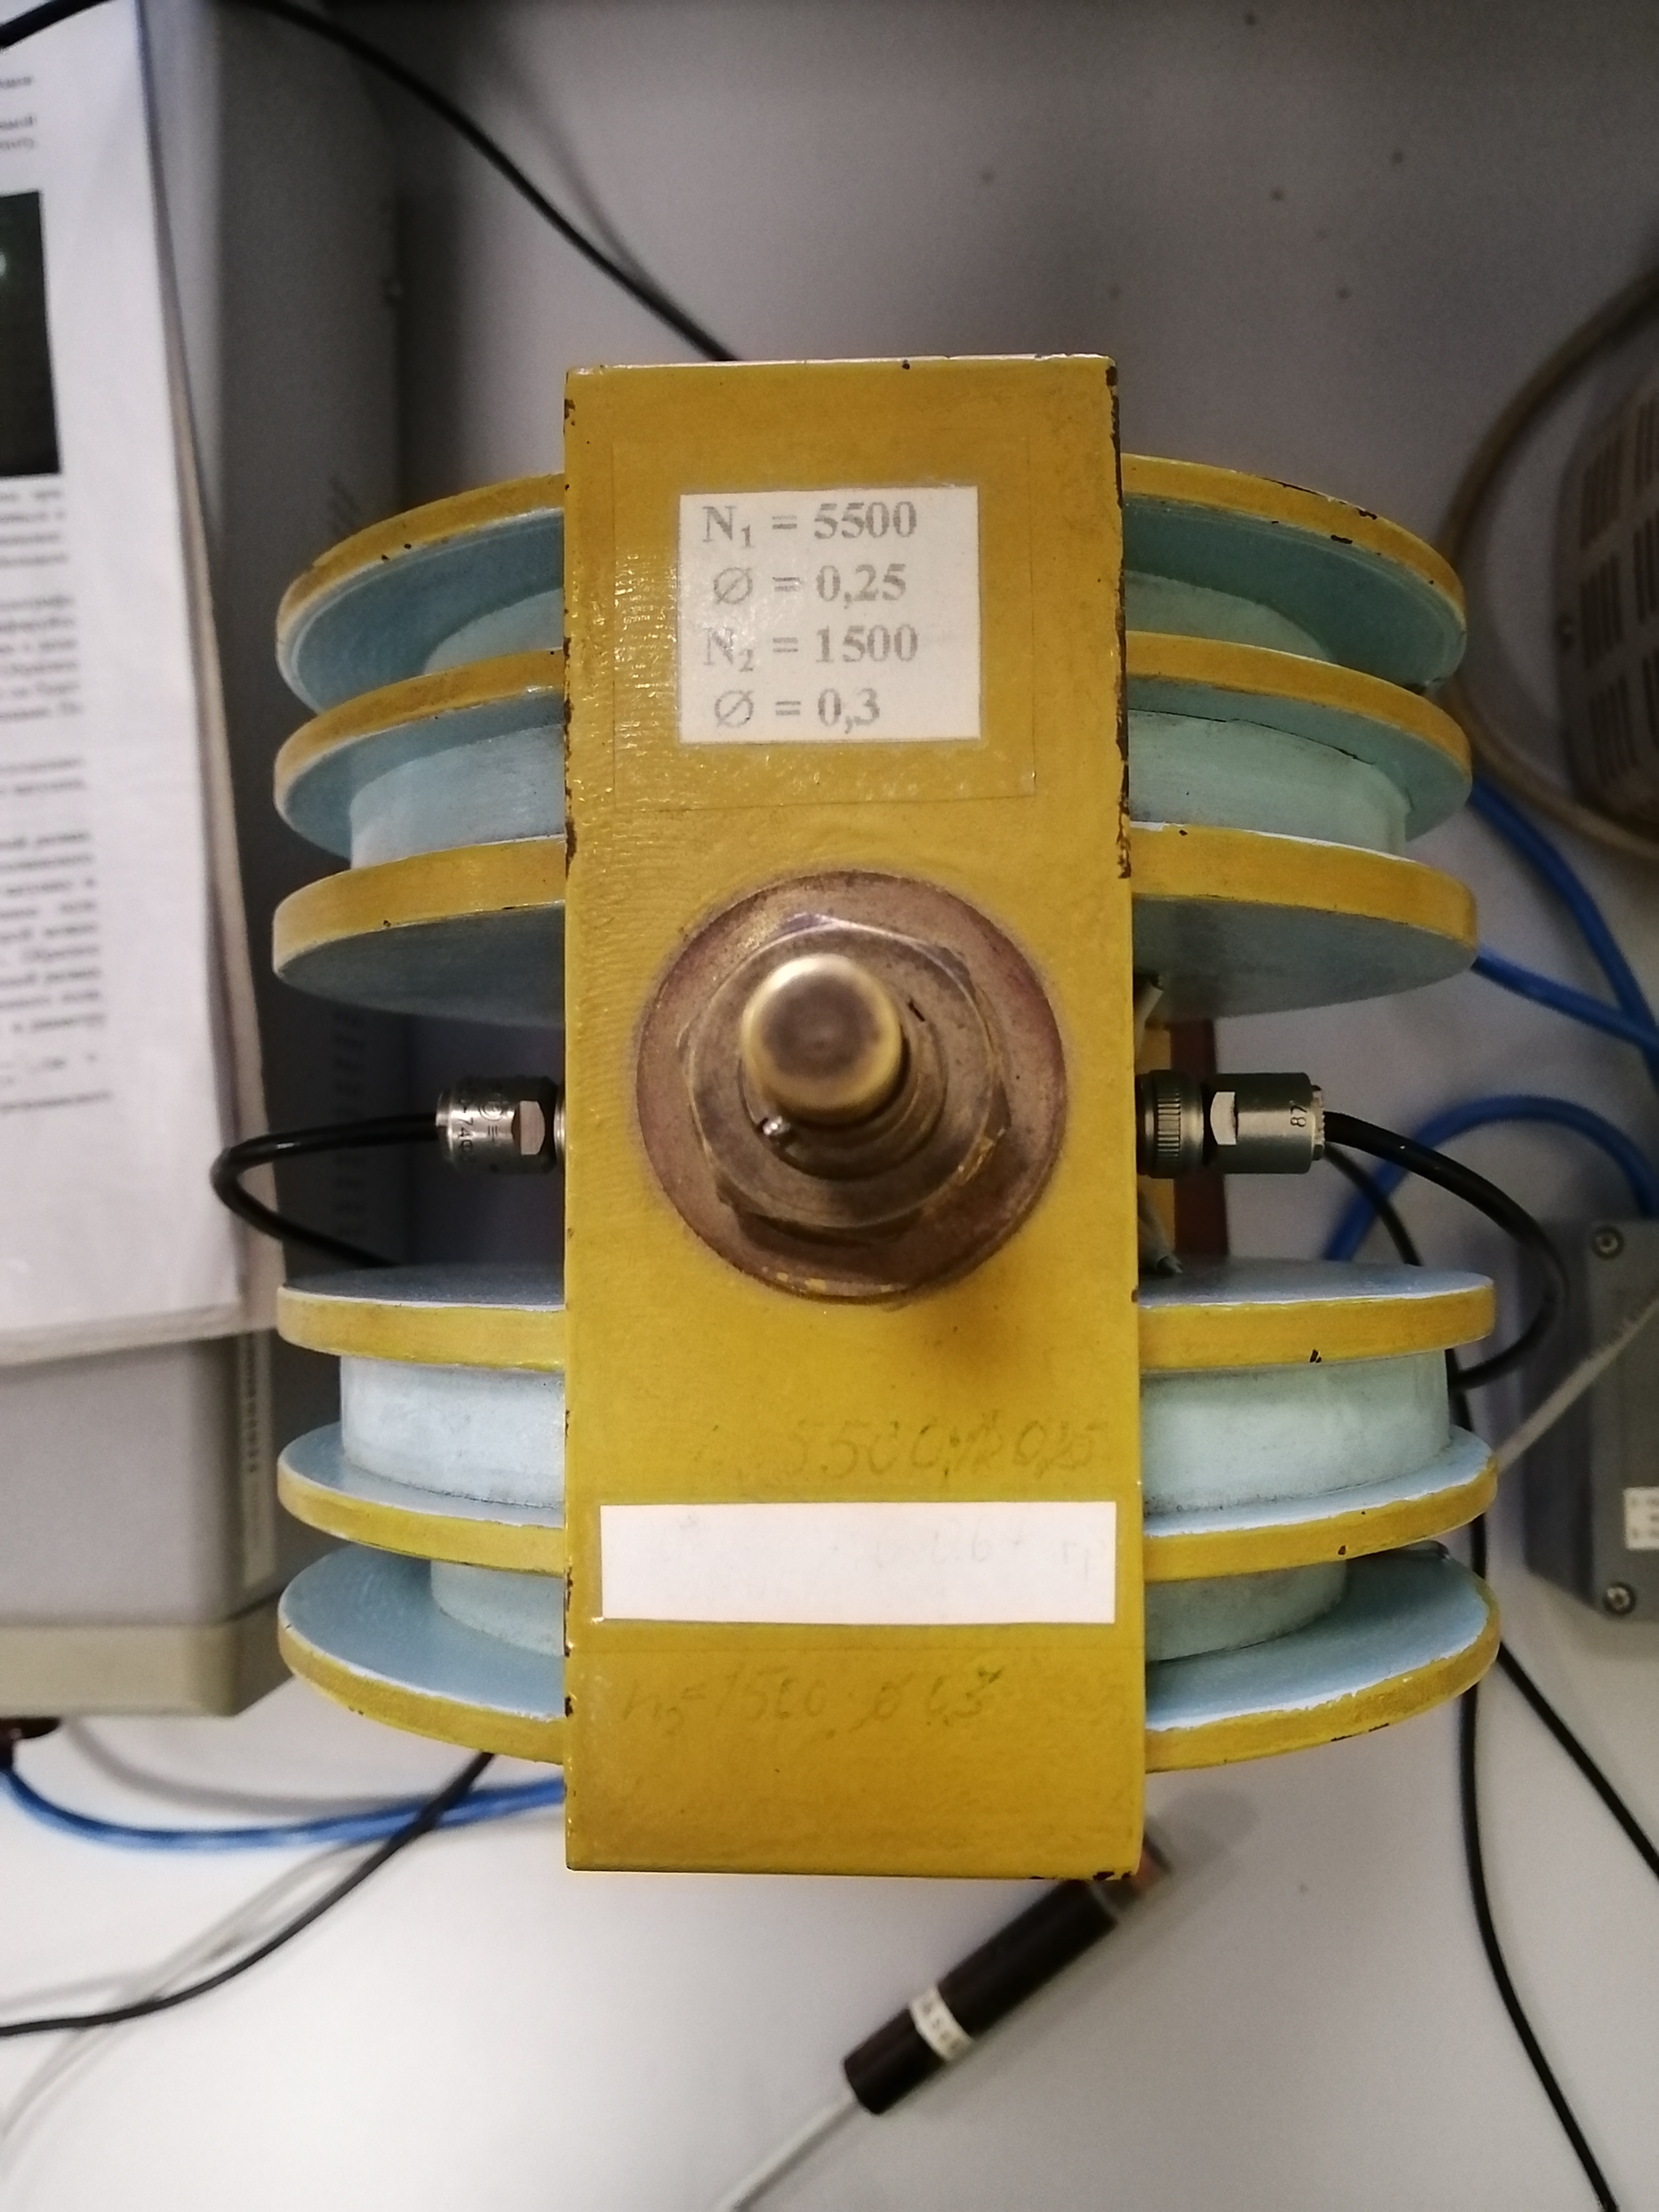
\includegraphics[width=0.7\linewidth]{photos/coil_top.jpg}
		\end{minipage}
		\caption{Центральная часть установки.}
		\label{fig:coil}
	\end{figure}
	
	Наблюдение ЭПР осуществляется измерением поглощения электромагнитного излучения, частота которого равна резонансной \eqref{eq:frequency}. Так как поглощение очень мало, необходимо сосредоточить энергию в объеме вещества. В нашей работе это достигается путем использования колебательного контура, в катушке которого расположена пробирка с веществом. Таким образом, при прохождении резонанса будет уменьшаться добротность катушки.
	
	На рис. \ref{fig:setup} приведена схема установки. Магнитное поле создается основными катушками, работающими от блока питания постоянного тока, и модулирующими катушками, работающими от ЛАТРа. Образец помещен в катушку колебательного контура радиоспектроскопа. Ось катушки перпендикулярна основному магнитному полю. Генератор МГц диапазона через петлю возбуждает колебания в контуре. Канал X осциллографа подключен к ЛАТРу, для получения развертки. Канал Y осциллографа через петлю связи измеряет колебания в контуре.
	
	\begin{figure}[H]
		\centering
		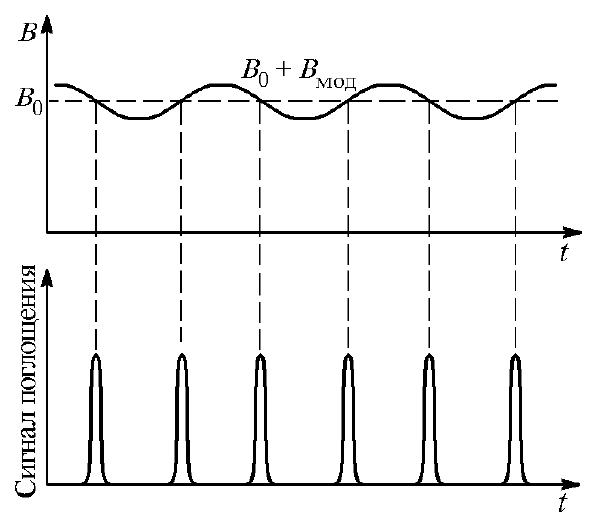
\includegraphics[scale=0.7]{res/signal.png}
		\caption{\centering
			 	 Сверху: зависимость основного поля от времени.\newline
			 	 Снизу: сигналы поглощения, снимаемые петлей связи.}
		\label{fig:metal}
	\end{figure}
	
	Частота генератора устанавливается в соответствии с \eqref{eq:frequency}. Емкость конденсатора колебательного контура настраивается изменением расстояния между пластинами. Таким образом частота колебательного контура уравнивается с частотой генератора. За счет модуляции основного поля два раза за период наблюдается точный резонанс, проявляющийся в увеличении сигнала на петле связи. Для удобства наблюдения измерения проводятся в режиме XY.
	
	\begin{figure}[H]
		\centering
		\begin{minipage}{0.5\textwidth}
			\centering
			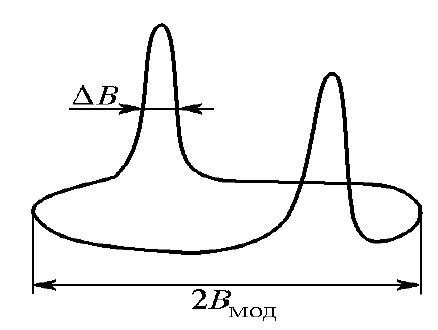
\includegraphics[width=0.9\linewidth]{res/xy.png}
		\end{minipage}%
		\begin{minipage}{0.5\textwidth}
			\centering
			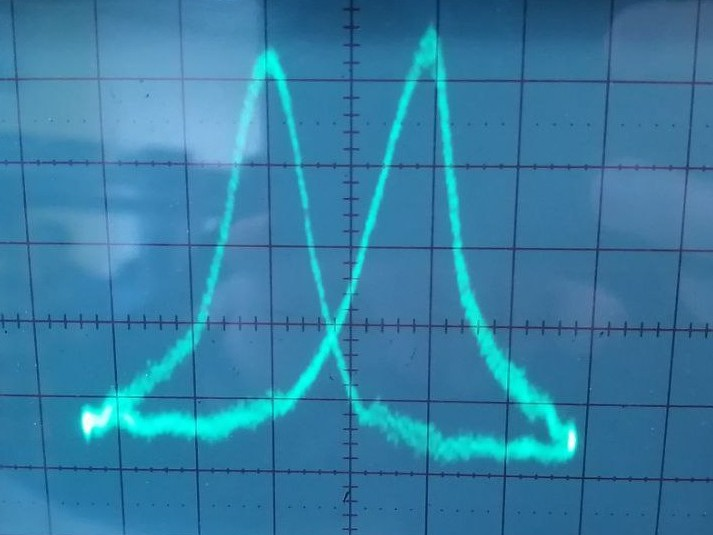
\includegraphics[width=1.0\linewidth]{photos/initial_setup.jpg}
		\end{minipage}
		\caption{Сигнал в режиме XY.}
		\label{fig:xy}
	\end{figure}
	
	Наличие двух сигналов за период объясняется фазовым сдвигом между напряжением и током модулирующих катушек. Для совмещения сигналов используется фазовращатель.
	
	Для градуировки шкалы осциллографа используем следующую технику: изменяем ток, текущий через основные катушки, пока пик ЭПР не сдвинется на две клетки вправо и влево, получая $V$, $V_{left}$, $V_{right}$.

	\section*{Результаты}
	
	\subsection*{Калибровка катушек}
	
	Для получения значений основного поля проводится калибровка. \textit{Основные} катушки подключаются к ЛАТРу для генерации переменного поля. Это поле снимается зондовой катушкой с известными параметрами: $N = 49$ витков, $d = (14.3 \pm 0.1)$ мм. Частота $f = 50$ Гц. Значения напряжений и поля являются действующими.
	
	$$V_{probe} = N B_0 \frac{\pi d^2}{4} 2 \pi f \quad \Rightarrow \quad B = \frac{V_{probe}}{N \frac{\pi d^2}{4} 2 \pi f}.$$
	
	\begin{figure}[H]
		\centering
		\begin{minipage}{0.4\textwidth}
			\centering
			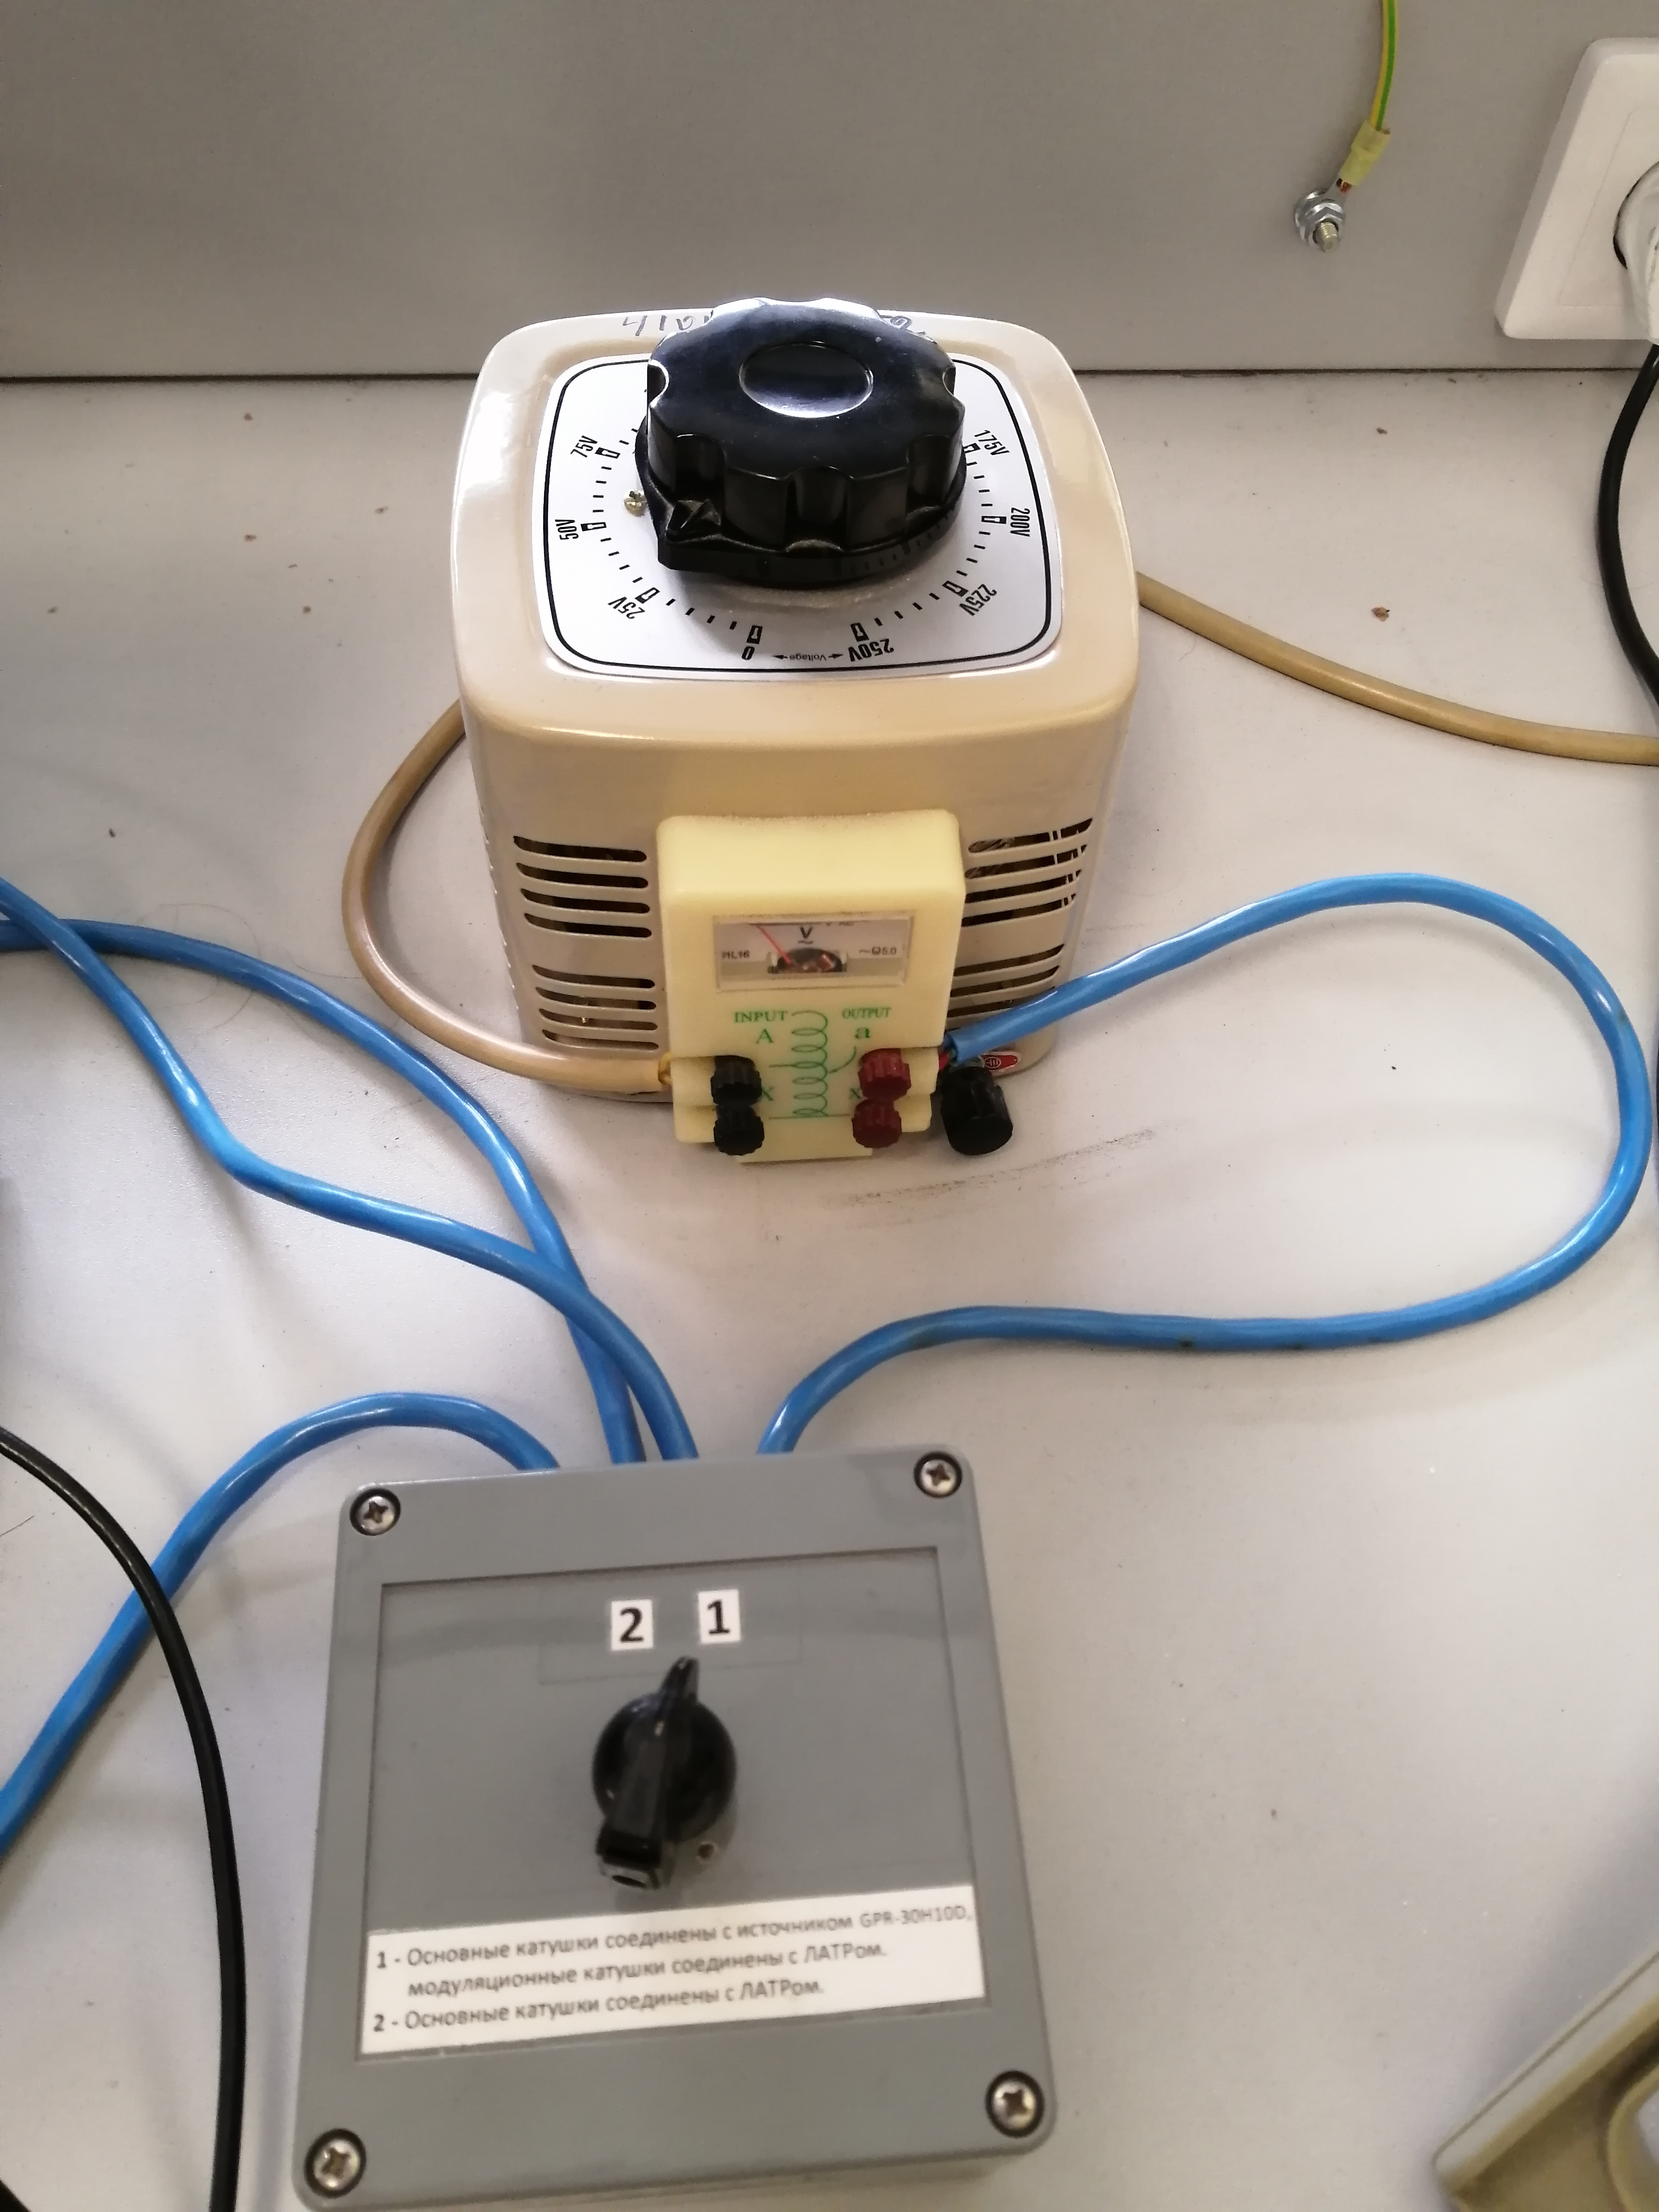
\includegraphics[width=0.7\linewidth]{photos/latr.jpg}
		\end{minipage}%
		\begin{minipage}{0.3\textwidth}
			\centering
			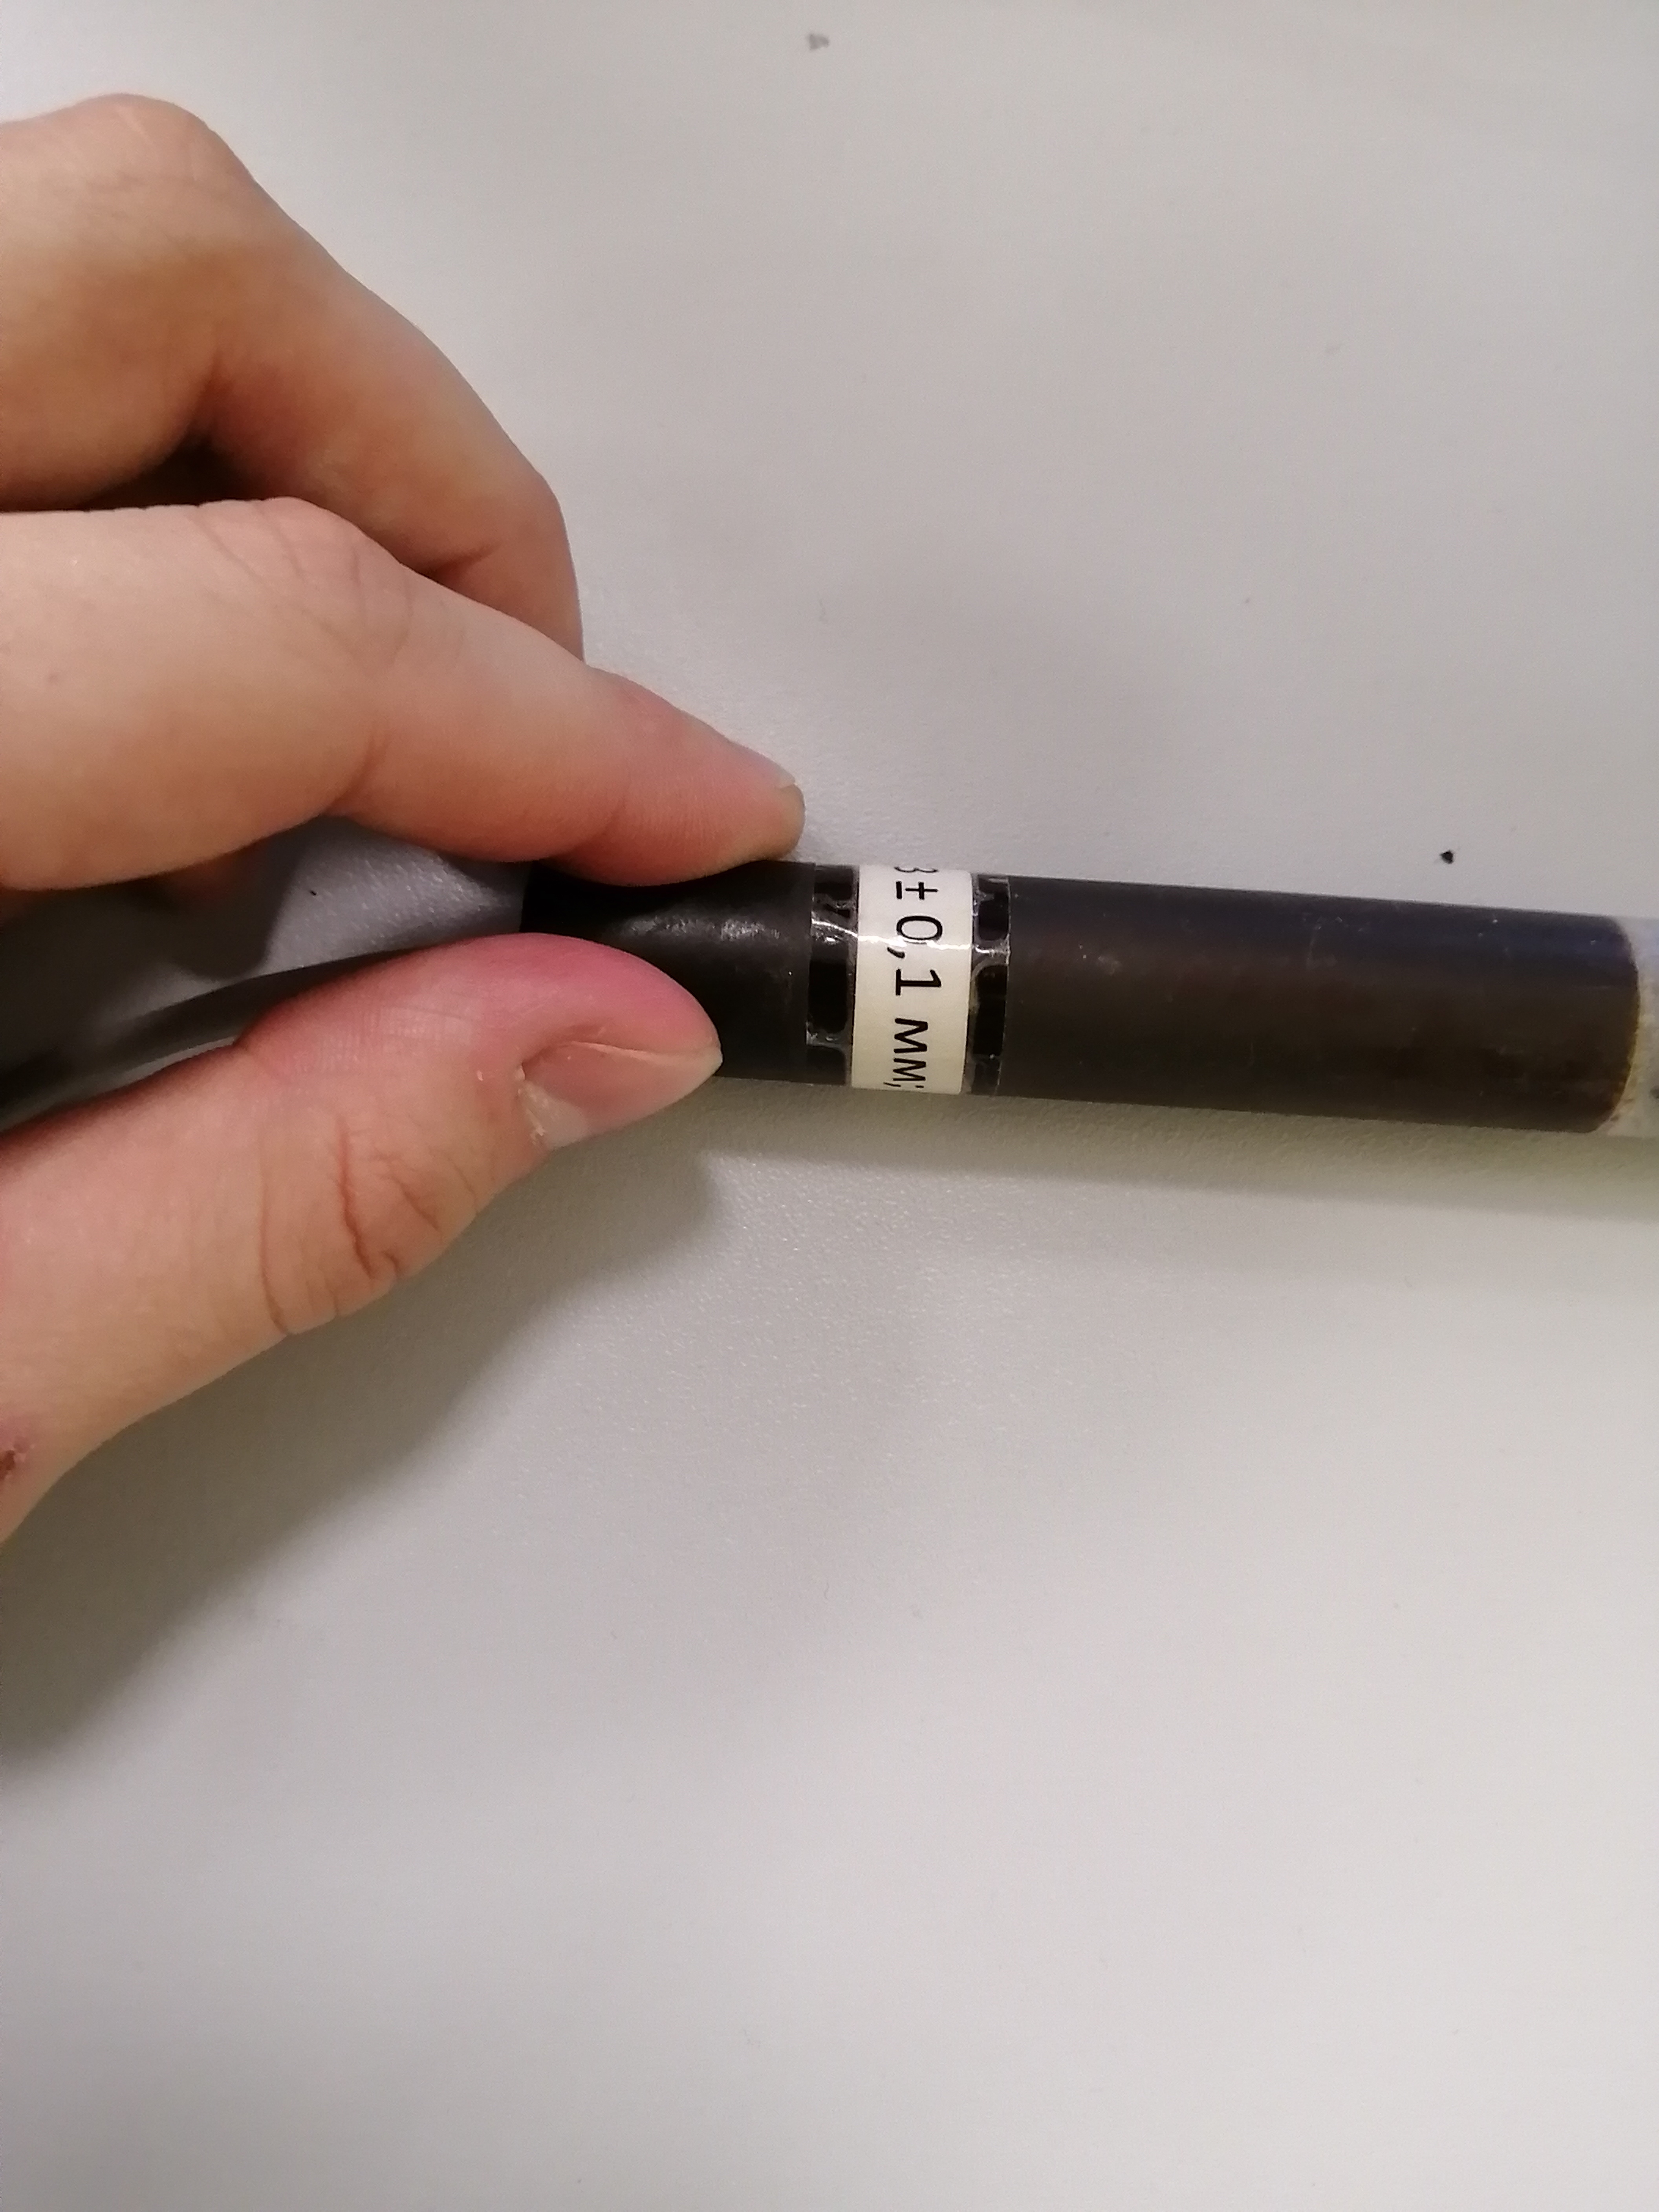
\includegraphics[width=0.7\linewidth]{photos/probe.jpg}
		\end{minipage}
		\caption{ЛАТР и зондовая катушка.}
		\label{fig:calibration_setup}
	\end{figure}
	
	\begin{minipage}{\textwidth}
		\begin{minipage}[]{0.7\textwidth}
			\centering
			\includegraphics[width=1.0\linewidth]{gen/calibration.pdf}
			\captionof{figure}{Зависимость поля от напряжения на измерительном резисторе.}
		\end{minipage}
		\hfill
		\begin{minipage}[]{0.29\textwidth}
			\centering
			\input{gen/calibration.tex}
			\captionof{table}{Данные калибровки катушек.}
		\end{minipage}
	\end{minipage}
	
	\subsection*{ЭПР}
	
	В соответствии с методикой, описанной выше, проведем измерения частоты $f$ электромагнитного излучения от напряжения на измерительном резисторе $V$. С помощью калибровки получим поля $B$. 
	
	\begin{table}[H]
		\input{gen/epr.tex}
		\caption{Измерения ЭПР.}
	\end{table}
	
	\begin{figure}[H]
		\centering
		\includegraphics[scale=0.9]{gen/epr.pdf}
		\caption{Зависимость частоты ЭПР от поля.}
		\label{fig:epr}
	\end{figure}
	
	Полученная зависимость линейна, что соответствует \eqref{eq:frequency}. Из наклона графика $k$ и \eqref{g_factor} определим:
	$$ g = \frac{\hbar k}{\mu_{\text{Б}}} = (1.94 \pm 0.04). $$
	
	Для ДФПГ $g$-фактор почти совпадает с $g$-фактором свободного электрона: $g_{ref} = 2.00$.
	
	\subsection*{Время релаксации}
	
	Для оценки времени релаксации получим значения ширины резонансных кривых.
	
	Воспользуемся значениями $V_{left}$, $V_{right}$ и калибровкой для получения деления осциллографа в единицах измерения поля.
	\begin{figure}[H]
		\centering
		\includegraphics[scale=0.8]{gen/widths.pdf}
		\caption{Значение одного деления осциллографа.}
		\label{fig:widths}
	\end{figure}
	
	$$ \Delta B = (2.36 \pm 0.15) \text{ Гс}. $$
	
	Определим ширины кривых в единицах поля.
	\begin{figure}[H]
		\centering
		\includegraphics[width=\linewidth]{photos/peaks.png}
		\caption{Резонансные кривые на разных частотах.}
		\label{fig:peaks}
	\end{figure}
	
	Рассчитаем время релаксации \eqref{eq:relaxation}:
	$$ \tau = \frac{\hbar}{2 \mu \Delta B} = (15.0 \pm 1.0) \text{ нс}. $$
	
	Справочное значение: $ \tau_{ref} \sim 60 \text{ нс}$, совпадает по порядку с полученнным в работе.
	\section*{Заключение и выводы}
	
	Работа подтверждает существование электронного парамагнитного резонанса.
	
	Получена зависимость \eqref{eq:frequency}, определено значение $g$-фактора для радикала ДФПГ: $g = (1.94 \pm 0.04)$, близкое к $g_{ref} = 2.00$
	
	По ширине резонансных кривых оценено время релаксации $\tau = (15.0 \pm 1.0)$ нс, совпадающее по порядку величины со справочным $\tau \sim 60$ нс.
	
\end{document}
